\documentclass{entry}

\title{卒業研究審査登録書の書式}
\author{G984822019}{吉村 直将}
\supervised{
	\supervisor{教授}{蓑原 隆}
	\supervisor{助手}{田島 信行}
}
\begin{document}
\maketitle

\section{はじめに(12ポイント)}
\subsection{研究背景}
近年,サイバー攻撃の発生件数が年々増加してきており,その攻撃手法も多様化している.過去の研究では,攻撃者を誘き寄せ,不正アクセスを受けるハニーポットを運用し,攻撃者の情報を収集してきた.攻撃者からハニーポットへの攻撃の流れとして図1に示してある.攻撃ホストはハニーポットにログイン試行としてID/パスワードを送信してくる.ハニーポットはそれに対して,ログイン許可をしている風に見せ,攻撃者はログイン後操作する為に,コマンドを送信する.この攻撃の中でハニーポットはログイン試行時に使われるIDやパスワード,ログイン後に攻撃者から送られるシェルコマンド等の情報を収集する,収集した情報から攻撃手法の研究をすることで,セキュリティ対策に繋げてきた. 
\begin{figure}[htbp]
	\centering
	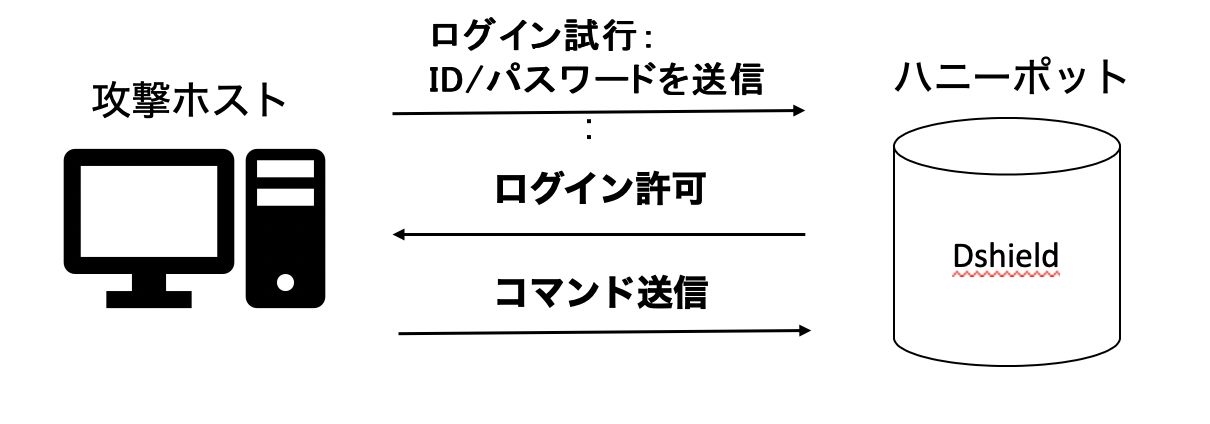
\includegraphics[width=\hsize]{honeypot.png}
	\caption{攻撃の流れ}
\end{figure}
\subsection{目的}
本研究では,攻撃者がログイン成功後に行われる攻撃手法に着目し、ハニーポットDshieldを用いて,攻撃者から送信されるコマンドやそのコマンドから入手できるファイルの情報を収集し,解析するシステムを構築し,攻撃の分析を行うことで,攻撃内容について警告を発することを目的とする。


\section{研究方法}
研究の方法
本研究では,ハニーポットDshieldを用いる.DShield(Distributed Intrusion Detection System)は,グローバルなセキュリティコミュニティによって構築された分散型侵入検知システムである.世界中のネットワーク上で発生するセキュリティイベントのデータを収集し,分析することでセキュリティの脅威情報を提供する.
Dshieldは研究室で以前から運用していたが,ログイン試行時のIdやパスワードを収集することを目的としたハニーポットであった.本研究では,ログイン後のコマンドを収集することが目的としている為,新しくハニーポットを構築することとする.         
研究計画として,
1.Dshieldを運用できる環境を構築をする。
2.コマンドを収集するために、Dshieldのプログラム内で、攻撃者からのコマンドに対してどうゆう動作をしているかを確認する。
3.実際にDshieldを運用してみる。
4.取集したコマンドの内容について調べる
5.コマンドからファイルURLなどを取集するプログラムを作成する。
6.ファイルがどのようなものなのか調べる
という手順っ進めていき、攻撃ファイルがどの様なものか把握し、警告を発する事で、セキュリティの向上に貢献したい.
これまでにできた事
新しくDshieldを構築した。
DshieldはCowrieというハニーポットが元になっていて、そのプログラムのログイン試行の攻撃に対するプログラムについてしらべた.
Dshieldを実際に運用してみて、コマンドを収集し、コマンド内容について調べた.

\section{今まで行ってきたこと}
\subsection{Dhieldの運用できる環境の構築}
\subsection{Dhieldが行う攻撃者のログイン試行への対処}
\subsection{収集したコマンド内容と攻撃者の意図}

A4縦方向で印刷できるように用紙のサイズを設定します.
上下左右の余白はそれぞれ,20,25,18,18mmです.
本文は2段組とし,段の間の空白は3文字分にします.

\section{今後やる事}



\bibliographystyle{entry}
%\bibliographystyle{junsrt}
\bibliography{sample}

\end{document}
